\documentclass[11.5pt]{article}
\usepackage[utf8]{inputenc}
\usepackage{amsmath,amssymb,amsthm,enumerate,float,geometry,latexsym,bm}
\usepackage{kpfonts}
\usepackage{hyperref}
\usepackage{apacite}
\usepackage{epigraph}
\usepackage{booktabs}
\usepackage{graphicx}
\usepackage{tikz}
\usepackage{caption}
\usepackage{multirow}

\usetikzlibrary{shapes.geometric,positioning}
\usepackage{pgfplots}
\usepackage[misc]{ifsym}

% Enhanced document geometry
\geometry{letterpaper, margin=1in}

% Spacing and paragraph formatting
\setlength{\parindent}{0.5in}
\setlength{\parskip}{6pt}
\linespread{1.5}

% Title and author information
\title{Doing Fabulous In Bad Times\footnote{From Dollar General's CEO quote ``We do very good in good times, and fabulous in bad times.''} \\ Dollar Store Expansion \& Nutritional Assistance}
\author{Alejandro Herrera-Caicedo }
\date{August 2024}

\begin{document}

% Title page
\maketitle
\begin{center}
\textbf{Draft version. Do not distribute or cite without permission.}
\end{center}

\begin{abstract}
    This paper investigates the supply-side effects of the Supplemental Nutritional Assistance Program (SNAP) on the entry of dollar stores, which simultaneously have rapidly expanded in low-income communities across the United States and typically offer food with low nutritional value. By analyzing the impact of SNAP policy changes, particularly the waiver of work requirements for able-bodied adults without dependents (ABAWD) in Virginia, the study finds a 15\% increase in dollar store entries in affected areas. Using a structural model, I show in a direct fashion that a dollar store faces a trade-off between opening nearby the distribution center and entering in a market with more SNAP users. I also show that in contrast with conventional retailers, the opening of a dollar store does not show signs of cannibalization. These patterns suggest that supply side reactions have the potential to undermine the desired outcomes of SNAP, for which I propose potential directions for evaluating policies currently under consideration by the Federal Government.
    
    
    %During the last decades dollar stores have significantly expanded in the U.S., predominantly serving to lower-income communities. This paper studies the role of policy distortions in driving the observed spatial distribution of dollar stores away from an efficient allocation. To provide empirical evidence of these inefficiencies, I estimate a model that integrates static demand estimation with a dynamic framework for store location decisions. I discuss the potential implications of this distortion to nutritional inequality, an issue of increasing concern in the U.S.
    
    
\end{abstract}


% Introduction -------------------------------------------------------------------------------------------------------------------------------
\section{Introduction}

% Literature Review ---------------------------------------------------------------------------------------------------------------------------
% 
In recent decades, dollar stores have expanded significantly, outpacing other food retailers. This rapid growth has become a pressing issue in public policy, as these stores disproportionately serve low-income households and, in some cases, are the only food retailers in the market. Both the literature and policymakers have primarily focused on how this expansion has crowded out local, healthier alternatives, potentially contributing to the phenomenon of food deserts in the United States. This shift may exacerbate the consumption of nutrient-poor foods among low-income households, a group that already suffers disproportionately from higher rates of hypertension, diabetes, cardiovascular diseases, obesity, and dental diseases \cite{shenkin2010using}. To aid lower-income households, policymakers have provided subsidies to households, most notably through the Supplemental Nutritional Assistance Program (SNAP), whose budget has nearly doubled from \$17 billion in 2000 to \$119 billion in 2022. While policymakers and academics have focused on how the subsidies act on the demand, the extent to which the supply side may react to this policy has remained understudied, even though the target audience of the assistance program is likely to overlap with the core consumer of dollar stores\footnote{On 2009 Nielsen's Research pointed out that 45\% of their consumer base are low-income households, that earn less than 30.000 a year \cite{nielsen2009dollarstores}}. As such, this article aims to provide evidence of how suppliers respond to the program, which would influence household choices and nutrition outcomes.


This article explores whether dollar stores' decisions to enter a market are influenced by the presence of SNAP households by asking two questions: Does the policy affect entry into the market? And if so, do dollar stores face a trade-off between entering nearby warehouses and markets with higher availability of SNAP households? By addressing these questions, the article sheds light on how unintended supply-side interactions with the policy might dampen the expected reach of the nutrition program.



To that end, I conduct two exercises. First, I provide reduced form evidence that the number of dollar stores increases when requirements for households to access SNAP are waived. Specifically, for an able-bodied adult without dependents (ABAWD) aged 18-49 to access SNAP, they must work at least 80 hours each month. In different years, the state of Virginia was granted the waiver of these requirements for some of its counties. It has been shown that this variation is important for SNAP access, as these work requirements significantly increase exits from incumbent beneficiaries by 64\% and reduce participation of potential beneficiaries by 53\% \cite{gray2023employed}. I exploit the staggered implementation of these waivers, finding that dollar store entry increases by 15\% after the waiver is enacted. However, this increase is not confined to dollar stores, as convenience stores exhibit a similar trend.



In the second exercise, I follow \citeauthor{holmes2011diffusion} \citeyear{holmes2011diffusion} to estimate a model with static demand and dynamic supply, where the consumers pre-allocate a budget to spend in an undisclosed dollar store, and the dollar store dynamically decides where to open its new stores. The model illustrates that counties with a higher share of households receiving SNAP benefits are more likely to shop at dollar stores. Consequently, the dollar store faces a trade-off between proximity to warehouses and being near SNAP users.

Additionally, the model measures cannibalization by quantifying the incremental sales, profits, and costs for each new store opening. In the analysis of Walmart, \citeauthor{holmes2011diffusion} showed that incremental sales decreased with the time since Walmart entered the market. In contrast, I find evidence against cannibalization, as it takes a considerable amount of time for a market to be saturated so that the incremental sales go down. While the lack of cannibalization is not surprising (these stores appear to serve a very local population), finding that less profitable stores are opening first suggest that there can be  underlying mechanisms at play that are beyond the scope of this paper. Potential explanations could be that dollar stores are engaging in pre-emptive entry\footnote{The literature on pre-emptive entry \cite{ellison2011strategic,gil2021preemptive} rationalize present value loses by arguing that a firm can opt to enter early into a \textit{medium} sized market with the intention of preventing competitors from entering.}, or a learning process of where to optimally allocate the stores. 


In the supply side estimation, the only unknown parameter is the distance to warehouses cost for which I won't provide a sharp confidence region. However, I do calculate a naive estimate of the parameter which serves two purposes: (1) provides an initial bound for the distance parameter, (2) a well-defined bound (i.e. implied lower bound is lower than the implied upper bound) serves as evidence of the trade-off between distance to warehouses and being nearby SNAP users: being further away from the distribution center and having access to more SNAP users entails a greater gross profit, but (mechanically) greater distribution costs. The opposite holds is also true. The naive estimate yields a well-defined bound, providing that the distribution costs are between 31.4 and 32.2 thousand dollars (2023) per 100 kilometers each year. 


The structural model employs data from multiple sources. The demand estimation relies on the aggregation of total sales, for which I use the volume of sales implied by the Kilts-Nielsen Scanner Data. I use demographics from the American Community Survey (ACS) at the county level. For the dollar store problem, I require the sequence of store openings, that I measured using the U.S. Department of Agriculture's SNAP Retailer Panel, which provides the exact geographic location of the dollar stores and the timing in which the store accepted SNAP's EBT payments. In addition to this, the supply required information on the sale's margins, the labor costs, and the land costs. The margins and labor-force are measured form the dollar store's reported 10K fillings, while the county's wages come from the County Business Patterns (CBP) payroll and employment measures in the retail industry, and rents are approximated using the residential rates from the ACS. 

This article contributes to three strands of the literature. First, to the works on the expansion of discount retail in the United States, and more specifically on the growing literature on the expansion of dollar stores and their effect on the retail landscape. Close to this article, there is  \citeauthor{caoui2022impact} \citeyear{caoui2022impact}, which has shown that dollar stores compete intensively in the food retail market, and that their entry is associated to the closure of competing stores, and the decline of consumption of fresh produce. Similarly,  \citeauthor{chenarides2021dollar} \citeyear{chenarides2021dollar} have shown the entry of dollar stores in food deserts increase the likelihood that they remain that way. Furthermore, \citeauthor{chenarides2024dynamic} \citeyear{chenarides2024dynamic} has shown that the entry of dollar stores crowds out small independent retailers. Interestingly, \citeauthor{schneier2023buck} \citeyear{schneier2023buck} do not find crowding out effects to dollar store entry, but do show that households tend to shop more on average at the dollar store. This article builds upon the literature, by distancing from the olipolistic concerns associated to the dollar store entry, and focusing more on the single-agent trade-offs that a dollar store faces when entering a market, pertaining to the economies of density (i.e. saving distribution cost by opening stores nearby distribution centers), and access to more SNAP beneficiaries.

Second, this research contributes to the literature on food access and nutrition. \citeauthor{allcott2019food} \citeyear{allcott2019food} conducted a structural analysis of nutritional inequality in the U.S., estimating a demand model for groceries. Their findings indicate that low-income households do not significantly shift their consumption towards healthier options even when they are presented with the same choices and prices as high-income households. 


Finally, regarding the literature on the impacts of SNAP on retail consumption, scholars have focused on the immediate implications of SNAP on household behavior. Closer to this article,  is \citeauthor{byrne2022welfare} \citeyear{byrne2022welfare} analysis of SNAP-approved retailers' stocking decisions, and consumer's purchasing choices, where SNAP-eligible households shift a small share of their consumption towards new SNAP retailers, and new SNAP stores offer a limited fresh inventory. Furthermore, works in public policy have discussed the effectiveness of SNAP, as it does not necessarily direct consumption toward healthy choices. \citeauthor{shenkin2010using} \citeyear{shenkin2010using} point that SNAP users disproportionately consume more carbonated drinks and estimated that in 2011 5\% of the SNAP expenditure was spent on carbonated soft drinks. Similarly, the USDA \citeyear{usdareport} reported that sweetened beverages are the second most purchased item by SNAP households, making up 9.3\% of their expenditure compared to 7.1\% for non-SNAP households. Conversely, the expenditure on fruits and vegetables by participating households was 11.9\%, while non-participating households spent 16.3\%. This reasoning has triggered an interest to making healthy food more attractive to SNAP users, as allowing for rebates for a narrow group of fruits and vegetables \cite{schanzenbach2017pros}. This article contributes to these works by examining the supply-side effects of SNAP on the retail landscape. The results suggest that if dollar stores are crowding out access to fresh produce and SNAP is incentivizing their entry, there are significant concerns about SNAP inadvertently undermining its own goals of improving nutritional outcomes. While I do not provide direct evidence that this is indeed happening, I highlight the potential issue for future research to address. Understanding these dynamics is crucial for policymakers and economists who aim to design more effective public assistance programs that truly enhance food access and nutritional equity.


The article is structured as follows: Section 2 provides the industry background, and Section 3 presents the data. Section 4 outlines the reduced form exercises that link SNAP to dollar store entry. Section 5 introduces the model, followed by the estimation procedure in Section 6, and the results in Section 7. Section 8 offers evidence on the lack of cannibalization, and Section 9 concludes.

\section{Industry Background}

\textit{Dollar Stores.} Over the past decade, dollar stores have become the fastest-growing food retailers in the United States. While these stores have existed since the mid-20th century, an increase in investment in distribution centers by 2010 allowed them to significantly outpace the more stagnant growth of supermarkets and supercenters. By 2019, dollar stores had closed the gap with grocery stores, which have been declining since 2013 \cite{caoui2022impact}. Notably, the top five brands comprise around 85\% of all dollar stores, with Dollar General, Dollar Tree, and Family Dollar being the largest. Additionally, Dollar Tree and Family Dollar merged in 2015, while allegedly still maintaining independent distribution centers and logistics\footnote{One of its institutional investors, Starboard Value LP, announced that ``Family Dollar and Dollar Tree banners have not truly been integrated and are largely run independently, both from a store operations and supply chain perspective.'' \cite{spglobal2024}}. There are instances where both stores co-exist as a ``combo store.'' Furthermore, the top three dollar store brands operate their own distribution centers.


Dollar stores are effectively discount retailer, offering a large variety of goods at a lower price than traditional retailers. The analysis of household expenditure by type of store done by \citeauthor{schneier2023buck} \citeyear{schneier2023buck} using Nielsen's Homescan (i.e. consumer panel data), shows that around 45\% of household expenditure on dollar stores falls in the consumption of baked goods, candy, carbonated beverages, cookies, juice and snacks. These are all goods that can be purchased with SNAP benefits. Furthermore, \citeauthor{caoui2022impact} \citeyear{caoui2022impact} have shown that their entry has been characterized by targeting locations that have significantly lower income per capita and rents, and a larger population that is black or below the poverty line. 



\textit{Supplemental Nutritional Assistance Program (SNAP).} The SNAP program, formally known as the Food Stamp Program, has existed in the United States since 1939, which was rebranded as the Supplemental Nutrition Assistance Program (SNAP) in 2008. The policy operates at a federal level, where the federal government pays for 100\% of the benefits, and the administrative costs are split with the local governments. The policy aims to low income households as the eligibility  has three criteria: (1) being at or below 130\% of the poverty line, or \$28550 a year, (2) net monthly income after deductions must be less than or equal to the poverty line, (3) assets cannot exceed certain limits. These criteria are more lenient for adults over the age of 60, and stronger for able-bodied adults without dependants (ABAWD). ABAWD can only access the program if they are working, otherwise they are limited to access the program for only three months. The amount that a household receives will depend on two factors: the number of members in the household, and the yearly maximum allotment policy, which are consistent across most states. For 2023 fiscal year, each member of a household will entail at most an additional \$219. 

%The program grants an estimated 175\$ per month per person \cite{usda2021snap}, and the provided value depends on the number of the household, 

The program provides eligible households with an Electronic Benefit Transfer (EBT) card, each month that can be spent on fruits and vegetables; meat, poultry, and fish; dairy products; bread and cereals; snack foods and non-alcoholic beverages; seeds and plants that can produce food. It cannot be used for alcoholic beverages, tobacco products, vitamins, or any nonfood item. 











% Data ---------------------------------------------------------------------------------------------------------------------------------------
\section{Data}

This article uses information from a large variety of sources, to adequately model demand and supply, and to provide reduce form evidence on the importance of SNAP. Concretely, I need information on the opening and location of stores and distribution centers, store sales, the demographic characteristics of each county, and the roll-out of the Virginia ABAWD waivers. 

The location and opening of stores are measured using the public Historical SNAP Retailer Locator Data. The SNAP Retail Data provides the universe of stores that accept SNAP benefits, when they started accepting the benefits, and where are they located up to the zip code and coordinates. Notably, this doesn't necessarily measure entry. This is notable during the second half of the 2000's when the number of dollar stores grew beyond what their financial reports announced. Fortunately, the growth is stabilized for the analysis period: 2012-2019. I retrieve the distribution center coordinates and opening from the dollar store's website, and local newspapers.

The sales of an undisclosed dollar store are computed using Kilts-Nielsen's Scanner data. This data provides weekly information on the volume of sales of 2.6-4.5 million Universal Product Codes (UPCs) including food, nonfood grocery items, health and beauty aids, and select general merchandise. All sales are aggregated at the store-year level, and later extrapolated to the universe of stores. This contrasts with other retail analysis that rely on census-level data of sales with a near-universe sample on a given year \cite{holmes2011diffusion}, or on multiple years \cite{ellickson2020measuring,chenarides2021dollar}. 


I also require information on the margins, labor demand and prices that the dollar store faces. I infer the margins and labor demand from the 10-K reports, which are only available from 2009-2015. I extrapolate the trend to the following years. For the input prices I use the county level average wages in the retail industry from the County Business Patterns, and the average residential rent from the American Community Survey. 

Finally, for the roll-out of the waiver of ABAWD requirements, I rely on the data provided by \citeauthor{gray2023employed} \citeyear{gray2023employed}, which details the fiscal-year and county-level implementation of ABAWD waivers in Virginia, identifying when and where these requirements were waived.

% Efforts are ongoing to locate distribution centers that complement this data. Secondly, demographic and SNAP participation data will be drawn from the American Community Survey, focusing on the Census Tract Level with 5-year binned data. Although yearly data is available for larger geographies, an extrapolation method will be applied to achieve finer granularity where necessary. Lastly, consumer expenditure patterns will be examined using the Kilts-Nielsen Consumer Panel data, providing insights into consumer spending behaviors.


% Reduced Form Evidence  ---------------------------------------------------------------------------------------------------------------------------------------
\section{Reduced Form Evidence}

A challenge of analyzing SNAP is that it is highly standardized across states. In this section, I provide evidence on how dollar stores in Virginia reacted to the waiving of SNAP's work requirements for able bodied adults without dependents (ABAWD). Starting in July of 2006, the State of Virginia allowed for the waiving of this requirement in different counties. The request was approved by the SNAP program as the counties for which the waiver was requested presented a higher unemployment than the national average. These requests allowed for a rollout where the variation falls in the timing of these waivers. After the great recession in 2009, the Recovery and Reinvestment Act (ARRA) exempted all counties from the ABAWD requirements, but requirements were imposed again on September 2013. After this, there was a second wave of waving exemptions from 2013 to 2019. It is note worthy that Virginia is not the only State where this happened, and that an ideal analysis would exploit the roll-out across the whole country. A desirable feature of this policy, is that the justification behind the policy is public, as a natural concern is that a State might request waivers when retailers enter a county\footnote{The ABAWD waiver information is provided by state \href{https://www.fns.usda.gov/snap/abawd/waivers}{on the Federal Nutrition Service website.}}. In this case, the waivers were requested and approved under the premise that these areas had an unemployment rate that was 20\% above the national average. 


The work of \citeauthor{gray2023employed} \citeyear{gray2023employed} uses a regression discontinuity approach that exploits both the roll-out of the policy and the age limit of the requirement (50 years old), to provide a convincing estimate on the effects of the re-instalment of requirements in adoption and remaining in the program. 
Here, I will be only using their data on the roll-out of the waivers to provide evidence on how limited access to the program affected the entry of dollar stores.  I estimate an event study equation for county $i$ at year $t$ from the year 2015 to 2019\footnote{I cannot study the first wave of the policy (2005-2014) as during these years dollar stores started accepting EBT payments, as such I will confound entry with retail enrollment.}:

\begin{align}
    \text{y}_{it} = \sum_{\tau = -3}^{4} \phi_\tau D^\tau_{it} + X_{it} \Lambda+ \zeta_{i} + \eta_t + \nu_{it}
\end{align}

Where $\text{y}_{it}$ is an approximation of the logarithm\footnote{As the distribution of dollar stores per county is zero-inflated I use the inverse hyperbolic sine transformation to approximate the logarithm.} of opening of dollar stores  in county $i$ at year $t$, $X_{it}$ are demographic characteristics, and $D_{it}^\tau$ is a dummy variable that activates if $t$ is $\tau$ years away from the requirement being waived. The $\zeta_i$ and $\eta_t$ are the county and year fixed effects. The vector of demographic characteristics aims to capture variables that would both explain entry and the policy taking place, for which I will control for the wage prices, the unemployment rate, the average income, and residential rates. As a robustness check, I estimate the model using \citeauthor{sun2021estimating} \citeyear{sun2021estimating}. In both specifications I cluster the errors at the county level. The results are presented in Figure \ref{fig:dollarStore}, showing an increasing pattern as the policy is enacted.  



\begin{figure}[h!]
    \centering
    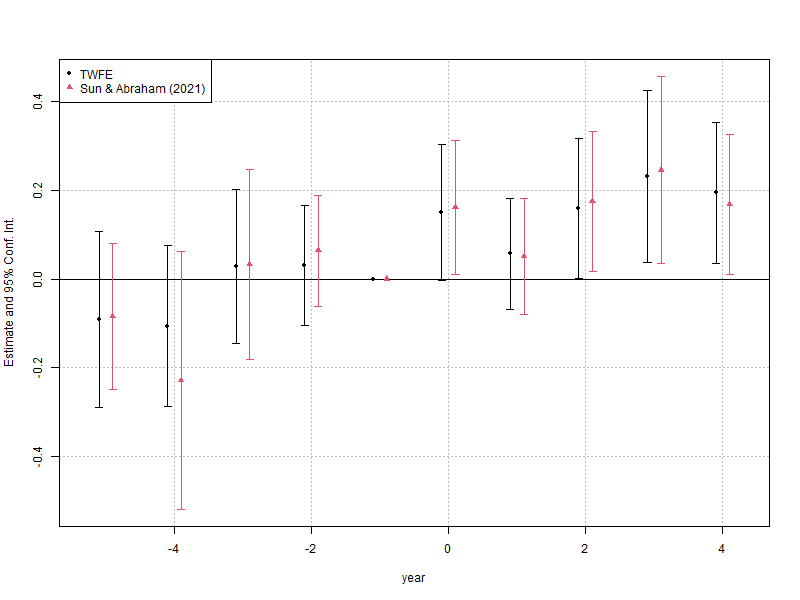
\includegraphics[width=0.75\linewidth]{Figures/se_all.ds_stores.png}
    \caption{Event Study - Number of Dollar Stores}
    \label{fig:dollarStore}
     \captionsetup{font=small, width=.75\textwidth}
\end{figure}


% \begin{figure}[h!]
%     \centering
%     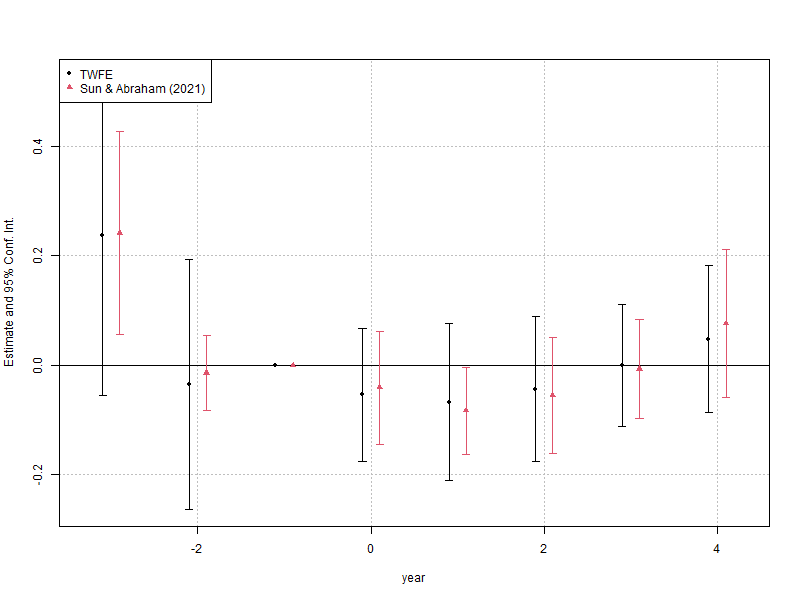
\includegraphics[width=0.75\linewidth]{Figures/se_all.nds_stores.png}
%     \caption{Event Study - Number of other Food Retailers}
%     \label{fig:nondollarStores}
% \end{figure}


Finally, I show on Table \ref{tab:regression} the average treatment effect implied by the Sun \& Abraham specification, finding that the roll-out is associated with 15\% more dollar store entries. I also show the results for other groups of stores, as Supermarkets, convenience stores, and multi-category. The results showcase that the increasing pattern is not unique to dollar stores, as Convenience Stores show a very similar pattern.
\input{Table/Regression.tex}



% Model ---------------------------------------------------------------------------------------------------------------------------------------
\section{Model}


Following the methodologies of \citeauthor{houde2023nexus} (2023) and \citeauthor{holmes2011diffusion} (2011), this study will focus on estimating the demand side and employing instrumental functions to delineate network trade-offs. The analysis will utilize demand estimates to (1) assess revenue impacts and cannibalization, and (2) determine the upper and lower bounds for the supply-side parameters.


\textit{Demand Side.} %As in \citeauthor{holmes2011diffusion} and \citeauthor{ellickson2020measuring}, the modeling and estimation of the consumer will rely on an observed expenditure, rather than on the market share. The modeling will stack the decission to buy into
This demand follows a similar specification to \citeauthor{holmes2011diffusion} (2011) and \citeauthor{ellickson2020measuring} (2020), where consumer decisions abstract away from price elasticities. Instead, a representative consumer is deciding how to spend each unit of budget 
pre-allocated to dollar-store expenditure. This aggregation allows for the estimation of the consumption primitives relying on sales data. The representative consumer of county $i$\footnote{It is possible to do this at a more granular scale, which is desirable to either have a more granular market, or to generate more variation across stores within one county.}, at year $t$, is deciding where to place a unit of expenditure $e$ among different alternatives  $s \in S_{t}\cup \{0\}$, where $S_t$ represents the available dollar stores in the market. The utility draws associated with each selection is characterized by:

\begin{align}
    u_{eist} =\tau_0 c_{is} + \tau_1 d_{is} z_{it} + \gamma_0 x_s + \gamma_1 x_s  z_{it} + \varepsilon_{eist} \notag\\  \quad \text{and} \quad  u_{ei0t} =  \beta_1w_{it}  + \beta_2 M_{it} + \varepsilon_{ei0t} \quad \varepsilon \overset{\text{i.i.d.}}{\sim} \text{T1EV}
\end{align}

The utility draws reflect that consumers lose utility from commuting, which is measured with $d_{it}$ being the distance of the store $s$ from the centroid of the county $i$. To introduce demographic-specific preferences, I will introduce a vector of demographics $z_{it}$ which will be interacted with the distance variable. For this analysis, the demographics include the share of SNAP enrollments and its interaction with average household size. It will also include average income, population, and vehicle access. Finally, I will introduce a vector of store characteristics $x_s$ which will capture preferences for the store characteristics, which will interact with the demographics.

%As it is conventional in this setting, the outside option is a function of the demographics $z_i$ and the population density $w_i$.  

 In the spirit of Holmes \citeyear{holmes2011diffusion}, the outside option is parameterized using the location characteristics $w_i$, which rely on an intercept, a second-order polynomial of the logarithm of the population density, and location characteristics, which in this case I set as the mean income. There are benefits from reviewing this specification so that it is more consistent with the inside option. An important weakness of this approach is that the outside option doesn't implicitly model the alternatives, as only one dollar store is present in the sales data. An ideal estimation would use census-like data to model the alternatives properly. I will deal with this in a reduced form way by introducing into the outside option utility $u_{ei0t}$ a vector with the number of retail competitors\footnote{In this vector I include other dollar stores and the retail firms analyzed by \citeauthor{ellickson2020measuring} \citeyear{ellickson2020measuring}, which include supermarkets, convenience stores, and multi-category brands (i.e. Walmart and Target).} $M_{it}$ and state-specific dummy variables. 

%To make up for this, I will provide an additional estimation by using each county's average income and the observed share of income destined for dollar stores.


Defining $\delta_{ist}$ as the deterministic part of the utility, we  have that the probability of allocating a unit of consumption on a store $s$ will be:

\begin{align}
    p_{ist} = \frac{\exp\{\delta_{ist}\}}{\sum_{s' \in S_t \cup \{0\}}\exp\{\delta_{is't}\} }
\end{align}

So that the expenditure of county $i$ in store $s$ at time $t$ will follow:

\begin{align}
     R_{ist}^\text{model}= \text{n}_{it} \times  \alpha \times  p_{ist} 
\end{align}

Where $\text{n}_{it}$ reflects the number of people living in county $i$ at time $t$. As such, $\alpha$ will represent the allocated budget for the dollar store, in thousands. As a store can only be in one county, I will drop the $i$ from revenue going forward. 


%The predicted revenues will be $R_s = \sum_{s \in \mathcal{S}_{it}} \alpha \times p_{ist} \times n_{it}$. Where $p_{ist}$ is the model's implied probability of selecting the store, and $\alpha$ is a parameter to estimate that captures the spending per consumer. With this, the parameters can be estimated using Maximum Likelihood by assuming that the difference between the modeled and observed revenue follows a normal or using Non-Linear Least Squares. 



\textit{Supply Side.} On the supply side I model the decision of \textit{where} to open stores. Importantly, the model abstracts away two important decisions: (1) how many stores to open in a given year, (2) how many distribution centers to build, and where to set them up. That is, the model takes these two decisions as given, and implicitly assumes separability on the payoffs of where to open the stores, and the number of stores and distribution center assortments. 


The supplier problem consists in a infinitely living, forward-looking, {Dollar Store} which endowed at $t=0$ with an assortment of stores $N_0$\footnote{The ideal model would use as t=0 the founding year of the dollar store. Because of data limitations, I take as 2012 as the starting year.}, and with an exogenous stock of warehouses, it maximizes its profit by selecting the sequence of store arrangements $\{N_t\}$, subject to the optimal number of store openings at year $t$:


\begin{align}
    \max_{\{N_t\}_{t=0}}\sum_{t=0}^\infty \beta^{t-1} \left(\bar \mu_t\sum_{s}   R_{st}(N_t) - C_t^\text{Dist}(N_t) - C_t^\text{Labor} (N_t) - C_t^\text{Land} (N_t) \right) \text{ subject to }  |N_t^*|-|N_{t-1}^*| 
\end{align}

 
 Going forward, I will call the firm's objective function $\Pi(N_t)$. In the objective function, $\bar \mu_t$ adjusts for the sales margins, and the two $C_t$ represent the distance and labor costs. In contrast with other analysis, as the construction of Walmarts, and Amazon distribution centers, I am distancing away from fixed costs. This is because dollar stores announce in their 10K Forms that most of their stores are leases, while Amazon and Walmart operate in a hybrid fashion. This is also done for convenience, as typically  the fixed costs are parameterized as a second order polynomial of the population density, entailing two additional parameters to estimate. As it is the convention, the firm faces linear distribution costs:

 \[C_t^{\text{Dist}}(N_t) = \lambda_d \sum_{s \in N_t}  d^\text{DC}_{s}\]
 
 Where $d_{s}^\text{DC}$ captures the distance to the closest distribution center to store $s$. It is noteworthy $\lambda_d$  is the only unknown parameter in the supply side. As I do not have information on the exact square footage of each store, I will rely on the average store square footage provided by the 10-K fillings ($F_t$) and the average rent price in each county:

 \[C_t^{\text{Land}}(N_t) =   F_t \sum_{s \in N_t}  r_{st}\]

 Similarly, I will use the average number of both full time and half time employees ($L_t$) provided in the 10-K, and the average wage in each county to characterize the cost function:

\[C_t^{\text{Labor}}(N_t) = L_t \sum_{s \in N_t}  w_{st}\]



 A well-known feature of this dynamic entry problem, is that the firm's problem has no known closed form solution, and that the firm's action space is incredibly large\footnote{That being said, there are known work-arounds that simplify the action space. \citeauthor{jia2008happens} \citeyear{jia2008happens} presents an algorithm to reduce the relevant action space of a static entry game by relying on the necessary conditions and lattice theory.}. For this, the solution will rely on revealed preference; the store arrangement in a particular year must yield a higher profit than a deviation.
 

 
 
 %Importantly, I have yet to parameterize $C_t^{\text{Labor}}$.
 
% Conclusion-----------------------------------------------------------------------------------------------------------------------------------
\section{Estimation}


\textit{Demand.} The estimation relies on observing the revenue of each store. One cannot match the sample of sales to the universe of stores. To approach this, I will run a LASSO regression and cross-validate to find the optimal penalization. The LASSO implementation serves to predict sales that are in counties out of sample, but also to predict distinct sales at the store level. I will heavily rely on the age of stores in the sales data, which will be observed imperfectly. The sampling will entail that the age in the sales data is underestimated, which I will assume it is a classical measurement error. Such measurement error entails that the variation within-county will be underestimated. 

With the predicted sales, the demand's parameters will be estimated using a non-linear least squares (NLLS). The routine aims for the demand specification to match the predicted sales:

\[\hat \theta_\text{1} = \arg \min_{\theta_1} \frac{1}{N} \sum_{s} \sum_{t \in T_s} \left( r^\text{model}(\theta_1;X_{sit})  - r^\text{data}_{st}\right)^2 \]

 Where the lowercase $r$ represents the logarithm of the respective sales levels. The objective functions is minimized by using the BFGS algorithm. Finally, for inference, I will use the bootstrap standard errors, as the asymptotic variance of NNLS can be unreliable in small samples \cite{hansen2022econometrics}.

%An important weakness of this approach is that the outside option doesn't implicitly model the alternatives, as only one dollar store is present in the data. An ideal estimation would use census-like data to model the alternatives properly. To make up for this, I will provide an additional estimation by using each county's average income and the observed share of income destined for dollar stores.


\textit{Supply.} This setting invites to find the set of parameters of $\lambda_d$ that would minimize the violated moment inequalities, which in this case are the deviations being preferred over the observed outcome. However, due to time constraints, I wont be able to do so. Instead, I will provide \textit{naive} bounds on the distance parameter ($\lambda_d$), which rely on finding the upper and lower bounds of a parameter by relying on instruments. This is the initial exercise executed by \citeauthor{houde2023nexus} \citeyear{houde2023nexus} to bound the distance parameter for Amazon's distribution. This exercise has two purposes: it provides a bound for the distance parameter, and provides initial evidence for the trade-off that the dollar store faces between reducing their costs and having access to a greater number of SNAP receivers. 


The inequalities that bound the parameters rely on the assumption of the dollar store being forward looking with perfect foresight, as it will entail deterministic inequalities where the observed opening of stores is better than the alternatives.  As in \citeauthor{holmes2011diffusion} (2010) and \citeauthor{houde2023nexus} (2023), the set of relevant inequalities will be achieved by the \textit{pairwise re-sequenced} inequalities introduced by  \citeauthor{bajari2005measuring} (2005) and \citeauthor{fox2007semiparametric} (2007). Namely, one would consider counterfactual networks composed by swapping the opening of a store $j$ with that of another store $j'$. By defining such a counterfactual sequence as $N^{jj'}$, from the observed one $N^*$, the implied inequality is:



\begin{align}
    m_N \equiv \Pi(N^*) - \Pi(N^{jj'}) + \epsilon^{jj'} \geq 0
\end{align}



   Where $\epsilon^{jj'}$ is a measurement error. A significant concern is the simultaneity between this error and the demand error, as there are likely unobservable affecting both. To address this concern, one should incorporate an instrumental variable that is not related to the error but is capable of capturing the trade-offs associated with the firm's maximization problem. In this setting, the objective is to use instrumental functions involving swaps that result in an increase in exposure to SNAP beneficiaries and an increase in cost distance to warehouses. The respective instruments are defined as:

   \begin{align}
       Z^{jj'}_1 = \mathbf{1}\{\Delta SNAP^{jj'} > 0, X_d^{jj'} > 0\} \quad \text{and} \quad  Z^{jj'}_2 = \mathbf{1}\{\Delta SNAP^{jj'} < 0, X_d^{jj'} < 0\}
   \end{align}

   Where the inputs of the instrument are characterized as:

     \begin{align*}
      \Delta SNAP^{jj'} & = \sum_{t=t(j)}^{t(j')} \beta^{t-1} \left( \sum_{s \in N_t^*} \frac{SNAP_{i_{(s)}t}}{SNAP_t}\right) -   \sum_{t=t(j)}^{t(j')} \beta^{t-1} \left( \sum_{s \in N_t^{jj'}} \frac{SNAP_{i_{(s)}t}}{SNAP_t}\right) \\
           X^{jj'}_d & =  \sum_{t=t(j)}^{t(j')} \beta^{t-1} \left( \sum_{s \in N_t^*}  d^\text{DC}_s \right)  -  \sum_{t=t(j)}^{t(j')} \beta^{t-1} \left( \sum_{s \in N_t^{jj'}} d^\text{DC}_s \right) 
  \end{align*}
  
   
   
  Where $SNAP_{i_{(s)}t}$ is the number of SNAP households in the county where store $s$ is located, at year $t$, while $SNAP_t$ is the total amount of SNAP households in year $t$, and $X^{jj'}_d$ as the discounted distribution distances. Furthermore, $t(j)$ and $t(j')$ refers to the entry date of store $j$ and $j'$ respectively. Under this structure, it is useful to separate the distance costs from the rest of the profit function. Define $Y^{jj'}$ as the difference in discounted gross profits of wages and rents between the observed outcome and the counterfactual outcome:

  \begin{align*}
      Y^{jj'} & =  \sum_{t=t(j)}^{t(j')}\beta^{t-1} \left(\bar \mu_t\sum_{s}   R_{st}^\text{model}(N_t^*)- C_t^\text{Labor} (N_t^*) - C_t^\text{Land} (N_t^*)\right)  \\
      & -  \sum_{t=t(j)}^{t(j')} \beta^{t-1} \left(\bar \mu_t\sum_{s}   R_{st}^\text{model}(N_t^{jj'}) - C_t^\text{Labor} (N_t^{jj'}) - C_t^\text{Land} (N_t^{jj'}) \right) 
  \end{align*}
  
  
  
  Using the revealed preference principle, one can provide an initial bound the distance primitive ($\lambda_d$) by relying on the instrument:
  


      \begin{align}
          \mathbb{E}[Y^{jj'}-\lambda_d X_d^{jj'} \mid Z^{1}_{jj'}] \geq 0 \iff \frac{\mathbb{E}[Y^{jj'}\mid Z^{1}_{jj'}]}{\mathbb{E}[X^{jj'}\mid Z^{1}_{jj'}]}\geq \lambda_d  \quad \text{and} \quad  \frac{\mathbb{E}[Y^{jj'}\mid Z^{2}_{jj'}]}{\mathbb{E}[X^{jj'}\mid Z^{2}_{jj'}]}\leq \lambda_d 
      \end{align}


    
     
     %If there is a trade-off between distance to warehouses and exposure to SNAP benefits, one would expect a change in expected gross revenues to follow this pattern: 
     
     
     %as the distance increases, expected gross revenues are anticipated to increase ($\mathbb{E}[Y^{jj'} \mid Z^{1}_{jj'}] > 0$), and as the distance decreases, expected gross revenues are anticipated to decrease ($\mathbb{E}[Y^{jj'} \mid Z^{2}_{jj'}] < 0$).
\newpage


\section{Estimation Results}
\textit{Demand.} The results show that the further a location is from the city’s centroid, the less likely a dollar store is to be selected. In line with the purpose of this article, the share of SNAP households in a county increases the likelihood that a household will select a dollar store. Additionally, in counties with larger households, it is less likely that a dollar store will be chosen. Finally, the model estimates that a representative household pre-allocates 730 dollars for dollar store expenditures (constant prices 2023). For comparison, the budget pre-allocated to Walmart is 2,633 dollars \cite{holmes2011diffusion}.

These results are consistent with the findings from the reduced-form analysis. In the model, the share of SNAP households drives sales upwards, as does household size. This sheds light on why dollar store entries respond to the waiver of ABAWD requirements, as this policy affects a very specific demographic. However, an important caveat is that the model fit has room for improvement. Potential avenues for this is to increase the granularity of the market, as some counties are significantly large making the choice set assumption unreasonable. Another alternative is to have a better grasp of the outside option, perhaps by fitting a moment on what is the household expenditure on retail. 



% Table created by stargazer v.5.2.3 by Marek Hlavac, Social Policy Institute. E-mail: marek.hlavac at gmail.com
% Date and time: Sun, Aug 04, 2024 - 9:01:20 PM
\begin{table}[!htbp] \centering 
  \caption{Demand Estimates} 
  \label{tab:demand} 
\begin{tabular}{@{\extracolsep{5pt}} lcc} 
\\[-1.8ex]\hline 
\hline \\[-1.8ex] 
Parameter &  & Value \\ 
\hline \\[-1.8ex] 
\textit{Preferences for the dollar store:}& & \\
\quad Distance from county centroid &  & -1.0353 \\ [-1.8ex] 
 &  & (0.0271) \\ 
\quad Share of households w/o vehicle  &  & -0.361 \\ [-1.8ex] 
 &  & (0.0148) \\ 
\quad Share of households with SNAP &  & 0.6255 \\ [-1.8ex] 
 &  & (0.0114) \\ 
\quad $\log$(Mean Income) &  & 0.2019 \\ [-1.8ex] 
 &  & (0.0116) \\ 
\quad $\log$(Mean Income) $\times$ distance &  & 0.8002 \\ [-1.8ex] 
 &  & (0.0184) \\ 
\quad Share of households w/o vehicle $\times$ distance  &  & 0.032 \\ [-1.8ex] 
 &  & (0.0234) \\ 
\quad  SNAP Share $\times$ distance  &  & -0.1728 \\ [-1.8ex] 
 &  & (0.013) \\ 
\quad Average Household Size &  & -0.0073 \\ [-1.8ex] 
 &  & (0.0107) \\ 
\quad  SNAP Share $\times$  Household Size &  & -0.4235 \\ [-1.8ex] 
 &  & (0.008) \\ 
\quad Distance $\times$  Household Size   &  & 0.1314 \\ [-1.8ex] 
 &  & (0.0187) \\ 
\quad Distance $\times$ SNAP Share $\times$ Household Size&  & 0.173 \\ [-1.8ex] 
 &  & (0.0125) \\ 
\textit{Preferences for the outside option:}& & \\
\quad Intercept &  & 3.6161 \\ [-1.8ex] 
 &  & (0.0688) \\ 
\quad $\log$(Population) &  & 2.0989 \\ [-1.8ex] 
 &  & (0.061) \\ 
\quad $\log$(Population)$^2$ &  & -1.0406 \\ [-1.8ex] 
 &  & (0.0234) \\ 
\quad  $\log$(Mean Income) &  & 0.1603 \\ [-1.8ex] 
 &  & (0.015) \\ 
\textit{Budget:}& & \\
\quad alpha &  & 0.73 \\ [-1.8ex] 
 &  & (0.0293) \\ 
 &  &  \\ 
 \hline
Objective Function &  & 0.1565 \\ [-1.8ex] 
R2 &  & 0.1068 \\ [-1.8ex] 
N &  & 66726 \\ 
\hline \\[-1.8ex] 
\end{tabular} 
 \captionsetup{font=small, width=.75\textwidth}
\caption*{Note: Bootstrapped standard errors in parenthesis. Sales measured in thousands of dollars (2023).}
\end{table} 




\newpage
\textit{Supply.} Table \ref{tab:supplybounds} provides the estimated upper and lower bound of $\lambda_d$. As highlighted by \citeauthor{houde2023nexus} \citeyear{houde2023nexus}, this estimate not only serves as an initial bound of $\lambda_d$, but also illustrates the trade-off that a dollar store faces when opening a store in terms of being close to the distribution center, but far away from SNAP benefits. The lower bound shows that a deviation that yields a greater exposure to SNAP, and a larger distance would yield a greater gross profit. On the other hand, being far away from the distribution center, but with greater access to SNAP users entails a larger gross profit. However, this must be interpreted carefully, as SNAP users and low wages are likely to be correlated, making it important to condition wages for a cleaner analysis. 


\begin{table}[ht]
\centering
\caption{Moment Conditions and Distance Trade-offs}
\begin{tabular}{lcccccc}
\toprule
 & \multicolumn{3}{c}{Lower bound: $\lambda_d$} & \multicolumn{3}{c}{Upper bound: $\lambda_d$} \\
& \multicolumn{3}{c}{$Z^{jj'}_2 = \mathbf{1}\{\Delta SNAP^{jj'} < 0, X_d^{jj'} < 0\}$}  & \multicolumn{3}{c}{$Z^{jj'}_1 = \mathbf{1}\{\Delta SNAP^{jj'} > 0, X_d^{jj'} > 0\}$}\\
\cmidrule(lr){2-4} \cmidrule(lr){5-7}
& N & $\mathbb{E}[Y\mid Z_2]$ & $\mathbb{E}[X_d\mid Z_2]$ & N & $\mathbb{E}[Y\mid Z_1]$ & $\mathbb{E}[X_d\mid Z_1]$ \\
\midrule
 &531,174 & -201.584 & -640.081 & 524,125 & 208.891 & 647.840 \\
\midrule
\multicolumn{2}{l}{{Bounds:} $\frac{E(Y|Z)}{E(X_d|Z)}$} &  & & \\
 & & 0.314 & & 0.322 \\
\bottomrule
\end{tabular}
 \captionsetup{font=small, width=.75\textwidth}
\caption*{Note: $\beta=0.95$. The profit function is estimated at an annual frequency, using thousands of dollars (2023). The distance units are measured in kilometers.}
\label{tab:supplybounds}

\end{table}


% \begin{table}[ht]
% \centering
% \resizebox{\textwidth}{!}{
% \begin{tabular}{lcccc}
% \toprule
%  & \multicolumn{2}{c}{Yield $(y_f)$} & \multicolumn{2}{c}{Revenue $(y_f\times p)$} \\
% \cmidrule(lr){2-3} \cmidrule(lr){4-5}
% & Action & Loss Condition & Action &  Loss Condition \\
% \midrule
% Individual&  $<$\textbf{c}overage,\textbf{p}rice$>$ & $y_f \lessgtr$ $\text{\textbf{c}} \times y$ & $<$\textbf{c}overage$>$ &  $y_f \times p  \lessgtr \text{\textbf{c}}  \times  \overline{y_f} $  \\
% Area & $<$\textbf{c}overage$>$  & $ \sum y_f \lessgtr \sum \text{\textbf{c}} \times \overline{y_f} $ & $<$\textbf{c}overage$>$  &  $ p \times \sum y_f \lessgtr \text{\textbf{c}} \times \overline{p} \times \sum \overline{y_f}$ \\
% \bottomrule
% \end{tabular}
% }
% \end{table}


%\newpage

\section{Preliminary Cannibalization Analysis}

In this section, I show preliminary evidence on the (lack of) cannibalization that the dollar stores experiences. The intuition is that an additional dollar store might "steal" the business from an incumbent store. To measure if this is happening, I will use the demand model to estimate for each store-year how much revenue and profit would have been lost if the store did not open. Formally, this is defined as the \textit{incremental sales} ($R^{inc}_{st}$) of store $s$ at year $t$. This analysis mirrors the one done for Walmart by \citeauthor{holmes2011diffusion} \citeyear{holmes2011diffusion}, which I complement by presenting the standard errors. This is also done for the profit, and the distance. Table 3 shows the average of these measures, binning them by the age of the first dollar store in the state. The point estimates highlight a lack of cannibalization, as incremental sales generally increase rather than decrease, which would be expected in the case of cannibalization. However, the increase in sales slows down as the first dollar store in the state ages.


The lack of cannibalization is consistent with the fact that dollar stores tend to flood a market, and that their scope is fairly local; in contrast with other retailers as Walmart, where people can do significant commutes to reach one. However, the fact that incremental profits go up entails that there might be an inter-temporal incentive that I am not capturing in the profit function. A potential explanation about this is that the dollar store might be engaging in pre-emptive entry, with the intention of keeping competitors at bay. This is an stylized behavior that has been studied for the drive-in-theaters and pharmaceutical industry \cite{gil2021preemptive,ellison2011strategic}, where a firms enter before in medium sized markets even if it is not profitable today, under the expectations that it will be profitable in the future if no one else enters the market.  The incremental distance shows that for the most part that the dollar store tends to build closer as the age of the first store increases. This trend reverses in the very last brackets, but with a smaller number of observations. 



\begin{table}[!htbp] \centering 
  \caption{Incremental Sales, Profit, and Distance} 
  \label{tab:cannibalization} 
    \resizebox{\textwidth}{!}{
\begin{tabular}{@{\extracolsep{5pt}} ccccccc} 
\\[-1.8ex]\hline 
\hline \\[-1.8ex] 
Age of first dollar store in the state &  N & Incremental Sales & Incremental Profit & Incremental Distance & Standalone Sales & Standalone Profit \\ 
\hline \\[-1.8ex] 
(0,2] & $155$ & 557.4622 & -2.1967 & 321.6786 & 10836.2319 & 306.1146 \\ 
 & $$ & (492.921) & (91.06) & (260.822) & (6809.27) & (1538.831) \\ 
(2,5] & $7,758$ & 670.0373 & 30.1794 & 263.9196 & 20944.2397 & 1741.549 \\ 
 & $$ & (498.452) & (103.739) & (234.836) & (29462.198) & (3586.625) \\ 
(5,10] & $35,692$ & 933.8895 & 91.4142 & 255.0566 & 37188.6534 & 6144.3877 \\ 
 & $$ & (631.714) & (139.943) & (197.268) & (62519.534) & (12485.961) \\ 
(10,15] & $25,148$ & 1076.1343 & 111.0255 & 256.1092 & 47925.9044 & 8604.3053 \\ 
 & $$ & (642.42) & (142.949) & (192.439) & (77337.381) & (15013.352) \\ 
(15,20] & $1,985$ & 1140.2772 & 127.328 & 293.0319 & 61090.3408 & 10720.4753 \\ 
 & $$ & (631.557) & (122.192) & (253.705) & (84717.29) & (15391.538) \\ 
(20,30] & $102$ & 1109.047 & 77.7555 & 597.3557 & 16221.2597 & 2258.019 \\ 
 & $$ & (704.403) & (136.944) & (308.097) & (10890.413) & (2376.745) \\ 
\hline \\[-1.8ex] 
\end{tabular}}
 \captionsetup{font=small, width=.95\textwidth}
\caption*{Note: Sales measured in thousands of dollars (2023). The distance unites are measured in kilometers. Standard errors in parenthesis.}
\end{table} 







% Conclusion-----------------------------------------------------------------------------------------------------------------------------------

\section{Conclusion}

The recent focus on food disparity has been accompanied by a significant increase in resources allocated to the SNAP program. In this article, I examine how this program also serves as an incentive for the entry of dollar stores, which have been linked by economists and policymakers\footnote{By 2024, there were an estimate of 60 communities trying to block the expansion \cite{businessinsider2024dollarstores}, among these Chicago, Illinois, took action in 2024, following Tulsa, Oklahoma, in 2018, Kansas City, Missouri, in 2016, and Mesquite, Texas, in 2019. The consequences of these policies are simulated by \citeauthor{caoui2022impact} \citeyear{caoui2022impact}.} to nutritional challenges, as they appear to displace healthier local alternatives in low-income markets, and have a role in the development of food deserts.  To demonstrate this, I conducted two key analyses.  First, I show that waiving work requirements for able bodied working adults (ABAWD) in Virginia entailed a 15\% increase in the number of entries of dollar stores, a pattern also observed with convenience stores. Next, I estimated a demand model and used this model to illustrate that dollar stores face a trade-off between opening near SNAP users or being closer to their distribution centers, with no significant evidence of cannibalization from new store openings. These results highlight that the dollar store reaction to SNAP has the potential to trump the program's effectiveness. However, while dollar stores have been stigmatized by not providing fresh produce, recently Dollar General (the largest chain in the market) has started to provide fresh produce in a quarter of its stores, a decision that warrants some analysis in the hope to exploit it in the benefit of lower income households. 

To what extent do dollar stores exploit the SNAP program to their own advantage and how can SNAP policy makers use this to the benefit of low income households? Recent policies against dollar store expansion and SNAP rewards for purchasing fresh produce\footnote{In the interest of enhancing the reach of SNAP, the federal government has run small pilots where households get rewarded when purchasing nutritious food. Namely, SNAP  participants in Massachusetts were randomly selected to have the option of requesting a rebate after purchasing a narrowly defined group of fruits and vegetables.} may push dollar stores in a new direction to provide healthier food to low-income households. In the light of this paper, future research could simulate the reach of these policies at a larger level, not only by analyzing changes in household consumption, but also on how supply reactions allow for the availability of healthier options. 

%Future research should incorporate how the supply side reacts to the program, and simulate the reach of this policy at a larger level, not only by analyzing changes in household consumption, but also on the availability of healthier options. Similarly, 

% In the interest of enhancing the reach of SNAP, the federal government has run small pilots where households get rewarded by a well defined group of vegetables and fruits. Future research could simulate the reach of this policy at a larger level, not only by analyzing changes in household consumption, but also on the availability of healthier options. Similarly, while dollar stores have been stigmatized by not providing fresh produce, recently Dollar General (the largest chain in the market) has started to provide fresh produce in a quarter of its stores, a decision that warrants some analysis in the hope to exploit it in the benefit of lower income households. 


% The growing ubiquity of dollar stores in the retail landscape for lower income household, has brought them to the attention of researchers and policy makers. This attention has focused on how the entry of dollar stores can end up crowding out of local, healthier options. This has been approached by local policy makers  by restricting their growth. 




% The firms involved in the analyzed case may be especially prone to collusion under common leadership. Taking the results seriously, we will do a back-of-the-envelope computation under the assumption that the coefficient is at most 10\% for the broader economy than what our preferred specification suggests (i.e. 1.2\%). We have that 1.2\% pairs of firms are at risk of engaging in collusion. If we are interested on the number of firms that are going to be invested in collusion, then: call $p$ the likelihood of not colluding, call $C$ the number of all firms that are connected to each other through a common leader, the expected number of firms affected by collusion would be:

% \[\sum_{c = 2}^{C} c \times \Pr(c) \]

% \


\newpage

\section{Appendix}

\subsection{Objective Function's Analytical Gradient}

The objective's function analytical gradient is required for the minimization routine. The objective function is:

\[f(\theta,X)= \frac{1}{N} \sum_S \sum_{T_s} (r_{sit}-\hat r(\theta,X_{it}))^2\]

There are three sets of parameters: the coefficient ($\alpha$) and the parameters for the inside ($\theta_I$) and outside options ($\theta_0$). The derivatives are:

\begin{align*}
    \frac{\partial f(\theta,X)}{\partial \alpha} &= -\frac{1}{N}\sum_I \sum_{T_i} 2(r_{sit} - \hat r_{sit}(\theta, X_{it})) \times \frac{1}{\hat R_{sit}(\theta,X_{it})}\times (n_i *  \hat \sigma_{sit}(\theta_I, \theta_0; X_{it}))\\
    \frac{\partial f(\theta,X)}{\partial \theta_0^k} & = -\frac{1}{N}\sum_I \sum_{T_i} 2(r_{sit} - \hat r_{sit}(\theta, X_{it}))  \times \frac{1}{\hat R_{sit}(\theta,X_{it})}\times  \left(n_i * \alpha *   \frac{\partial \hat\sigma_{sit}(\theta_I, \theta_0; X_{it})}{\partial \theta_0^k}\right) \\
    \frac{\partial f(\theta,X)}{\partial \theta_I^k} & = -\frac{1}{N}\sum_I \sum_{T_i} 2(r_{sit} - \hat r_{sit}(\theta, X_{it}))  \times \frac{1}{\hat R_{sit}(\theta,X_{it})}\times  \left(n_i * \alpha *   \frac{\partial \hat\sigma_{sit}(\theta_I, \theta_0; X_{it})}{\partial \theta_I^k}\right) 
\end{align*}

The derivatives of the share are:


\begin{align*}
    \frac{\partial \hat\sigma_{sit}(\theta_I, \theta_0; X_{it})}{\partial \theta_0^k} &  = - x^0_{k,it} \hat \sigma_{sit}(\theta,X_{it}) \hat \sigma_{0it}(\theta,X_{it}) \\
    \frac{\partial \hat\sigma_{sit}(\theta_I, \theta_0; X_{it})}{\partial \theta_I^k} & = \hat \sigma_{sit}(\theta, X_{it})  \left(x_{k,sit}^I - \sum_{s'} x_{k,s'it}^I \hat \sigma_{s'it}(\theta, X_{it})\right)
\end{align*}

% In vector form:

% \begin{align*}
%     \frac{\partial \hat\sigma_{sit}(\theta_I, \theta_0; X_{it})}{\partial \theta_0} &  = - X^0_{it} \odot [\hat \sigma_{sit}(\theta,X_{it}) *  \hat \sigma_{0it} (\theta,X_{it})]\\
%     \frac{\partial \hat\sigma_{sit}(\theta_I, \theta_0; X_{it})}{\partial \theta_I} &  =  \hat \sigma_{sit}(\theta, X_{it}) \times  \left(X^I_{sit} - (X^I_{it})^\top \cdot \hat \sigma_{it} (\theta, X_{it}) \right)
% \end{align*}
% \newpage

% The second derivatives are:

% \begin{align*}
%      \frac{\partial^2 f(\theta,X)}{\partial \alpha^2} & = 0 \\
%      \frac{\partial^2 f(\theta,X)}{\partial \alpha \partial \theta_0^k} & =  -\frac{1}{N}\sum_I \sum_{T_i} 2(r_{sit} - \hat r_{sit}(\theta, X_{it}))  \times \frac{1}{\hat R_{sit}(\theta,X_{it})}\times  \left(n_i *   \frac{\partial \hat\sigma_{sit}(\theta_I, \theta_0; X_{it})}{\partial \theta_0^k}\right) \\
%      \frac{\partial^2 f(\theta,X)}{\partial \alpha \partial \theta_I^k} & =  -\frac{1}{N}\sum_I \sum_{T_i} 2(r_{sit} - \hat r_{sit}(\theta, X_{it}))  \times \frac{1}{\hat R_{sit}(\theta,X_{it})}\times  \left(n_i *   \frac{\partial \hat\sigma_{sit}(\theta_I, \theta_0; X_{it})}{\partial \theta_I^k}\right) \\
%      \frac{\partial^2 f(\theta,X)}{\partial \theta_0^k \partial \theta_I^{k'}} & =  -\frac{1}{N}\sum_I \sum_{T_i} 2(r_{sit} - \hat r_{sit}(\theta, X_{it}))  \times \frac{1}{\hat R_{sit}(\theta,X_{it})}\times  \left(n_i * \alpha*  \frac{\partial^2 \hat\sigma_{sit}(\theta_I, \theta_0; X_{it})}{\partial \theta_0^k \partial \theta_I^{k'}}\right) \\
%      \frac{\partial^2 f(\theta,X)}{\partial \theta_0^k \partial  \theta_0^{k'}} & =  -\frac{1}{N}\sum_I \sum_{T_i} 2(r_{sit} - \hat r_{sit}(\theta, X_{it}))  \times \frac{1}{\hat R_{sit}(\theta,X_{it})}\times  \left(n_i * \alpha*  \frac{\partial^2 \hat\sigma_{sit}(\theta_I, \theta_0; X_{it})}{\partial \theta_0^k \partial  \theta_0^{k'}}\right)\\
%      \frac{\partial^2 f(\theta,X)}{\partial \theta_I^k \partial \theta_I^{k'}} & =  -\frac{1}{N}\sum_I \sum_{T_i} 2(r_{sit} - \hat r_{sit}(\theta, X_{it}))  \times \frac{1}{\hat R_{sit}(\theta,X_{it})}\times  \left(n_i * \alpha*  \frac{\partial^2 \hat\sigma_{sit}(\theta_I, \theta_0; X_{it})}{\partial \theta_I^k \partial  \theta_I^{k'}}\right)
% \end{align*}

% The second derivative for the share entails:


% \begin{align*}
%    \frac{\partial^2 \hat\sigma_{sit}(\theta_I, \theta_0; X_{it})}{\partial \theta_0^k \partial \theta_I^{k'}} & = - x_{k,it}^0 \left[\frac{\partial \hat \sigma_{sit}}{\partial \theta_I^{k'}} \hat \sigma_{0it} -  \hat \sigma_{sit}  \hat \sigma_{0it} \sum_{s'} x_{s'it}  \hat \sigma_{s'it}  \right] \\
%   \frac{\partial^2 \hat\sigma_{sit}(\theta_I, \theta_0; X_{it})}{\partial \theta_I^k \partial \theta_I^{k'}} & = \frac{\partial \hat \sigma_{sit}}{\partial \theta_I^{k'}}  \left(x^I_{k,sit} -  \sum_{s'} x_{k,s'it}^I \hat \sigma_{s'it}\right) + \hat \sigma_{sit} \sum_{s'} x_{k,s'it}^I \frac{\partial \hat \sigma_{s'it}}{\partial \theta_{I}^{k'}}\\
%   \frac{\partial^2 \hat\sigma_{sit}(\theta_I, \theta_0; X_{it})}{\partial \theta_0^k \partial \theta_0^{k'}} & = - x_{k,sit}^0 \left(\frac{\partial \hat \sigma_{sit}}{\partial \theta_0^{k'}} \hat \sigma_{0it}  + x_{k',it}^0 \hat  \sigma_{sit} \hat \sigma_{0it} (1- \hat \sigma_{0it}) \right)
% \end{align*}



% \newpage
% The algebra is:
% \begin{align*}
%     \frac{\partial \hat\sigma(\theta_I, \theta_0; X_{it})}{\partial \theta_0^k} & = \frac{-\exp(\theta_{I}X_{it}^I) x^0_{k,it} \exp(\theta_0 X_{it}^0) }{\left(\exp(\theta_0 X_{it}^0) + \sum_j \exp(\theta_I X_{jt}^I)\right)^2} = - x^0_{k,it} \hat \sigma(\theta,X_{it}) \hat \sigma(\theta,X_{0t}) \\
%     \frac{\partial \hat\sigma(\theta_I, \theta_0; X_{it})}{\partial \theta_I^k} & = \frac{x^I_{k,it} \exp(\theta_I X_{it}^I) \times \left(\exp(\theta_0 X_{it}^0) + \sum_j \exp(\theta_I X_{jt}^I)\right) - \exp(\theta_I X_{it}^I) \sum_{j}( x_{jt}^I \exp(\theta_I X_{jt}^I))}{\left(\exp(\theta_0 X_{it}^0) + \sum_j \exp(\theta_I X_{jt}^I)\right)^2} \\
%     & = x_{k,it}^I \hat \sigma(\theta, X_{it}) -  \hat \sigma(\theta, X_{it}) \left(\sum_j x_{jt}^I \hat \sigma(\theta, X_{jt})\right)\\
%     & = \hat \sigma(\theta, X_{it})  \left(x_{k,it}^I - \sum_j x_{jt}^I \hat \sigma(\theta, X_{jt})\right)
% \end{align*}





% References
\newpage
\bibliography{references}
\bibliographystyle{apacite}

\end{document}
